\subsection{State variable feedback}\label{chapter_StateVariableFeedbackIMPL}

It is no problem for a state space controller to move the poles wherever the engineer wants them to go. How to do this by hand is explained in chapter \ref{chapter_PolePlace}. For this much more complicate process MATLAB is used. In chapter \ref{chapter_PolePlacementIMPL} the decision to move the poles to [-18 -5 -7 -10 -9] is made. As mentioned, MATLAB is used to find the state variable feedback factors needed by the state space controller to move the poles to the specific position. The following code calculates them.

\begin{lstlisting}
System = linmod('dynamics_reduced_without_motordelay');
StateSpace = ss(System.a, System.b, System.c, System.d);
K_ret = place(System.a, System.b, [-18 -5 -7 -10 -9]);     
\end{lstlisting}

The function place() calculates the state variable feedback factors. The result is:

\begin{align}\label{eq:feedback}
\bordermatrix[{[]}]{
	  				&  rpsi & theta & phi & rphi & rtheta \cr
rpsi\_set 	&  7.27 & 0 & -0.57 & -0.07 & 0.03 \cr
theta\_set	&  0.76 & 79.36 & 0.03 & 0 & 20.28 \cr
phi\_set		& 0 & 0 & 65.05 & 15.80 & 0 \cr
}
\end{align}

This matrix describes with which gain, which state variable has to be fed back. For example the state variable theta has to be fed back with a gain of 20.28 to the theta\_set path. 

There are two ways to prove, that the poles are moved to the estimated places. The first way is, to calculate the closed loop state matrix and the output matrix with the calculated feedback factors. The following code is doing that.

\begin{lstlisting}
A_CL = System.a - System.b * K_ret;
C_CL = System.c - System.d * K_ret;
Sys_ClosedLoop = ss(A_CL, System.b, C_CL, System.d);
eig(Sys_ClosedLoop)
\end{lstlisting}

The output of the eig() function are the poles that are passed to the place() function earlier. So it is clear, that the poles now are, where they should be. 

The second way is, to create the closed loop Simulink block diagram and get the state space representation with linmod(). At this point it is also possible to check weather it was a good or a bad decision to ignore the motor delays. The Simulink block diagram used in the following includes the whole state space controller and the process. Furthermore the motors with delay are used.

\begin{lstlisting}
S_CL = linmod('ControllerAndProcess');
SS_ClosedLoop = ss(S_CL.a, S_CL.b, S_CL.c, S_CL.d);
eig(SS_ClosedLoop)
\end{lstlisting}

And like expected, the result is:

\begin{lstlisting}
-9,66
-7,13
-4,99
-9,07
-18,47
-1016
-991
-977
-1000
\end{lstlisting}

The first five poles are the expected poles - not exactly, but a good result. The four remaining poles are those for the motor delays. So it is possible to see, that they do not really disturb the others, because they are very far away on the left side of the s-plane.


So how does this feedback look like in a Simulink block diagram? 

\begin{figure}
	\centering
		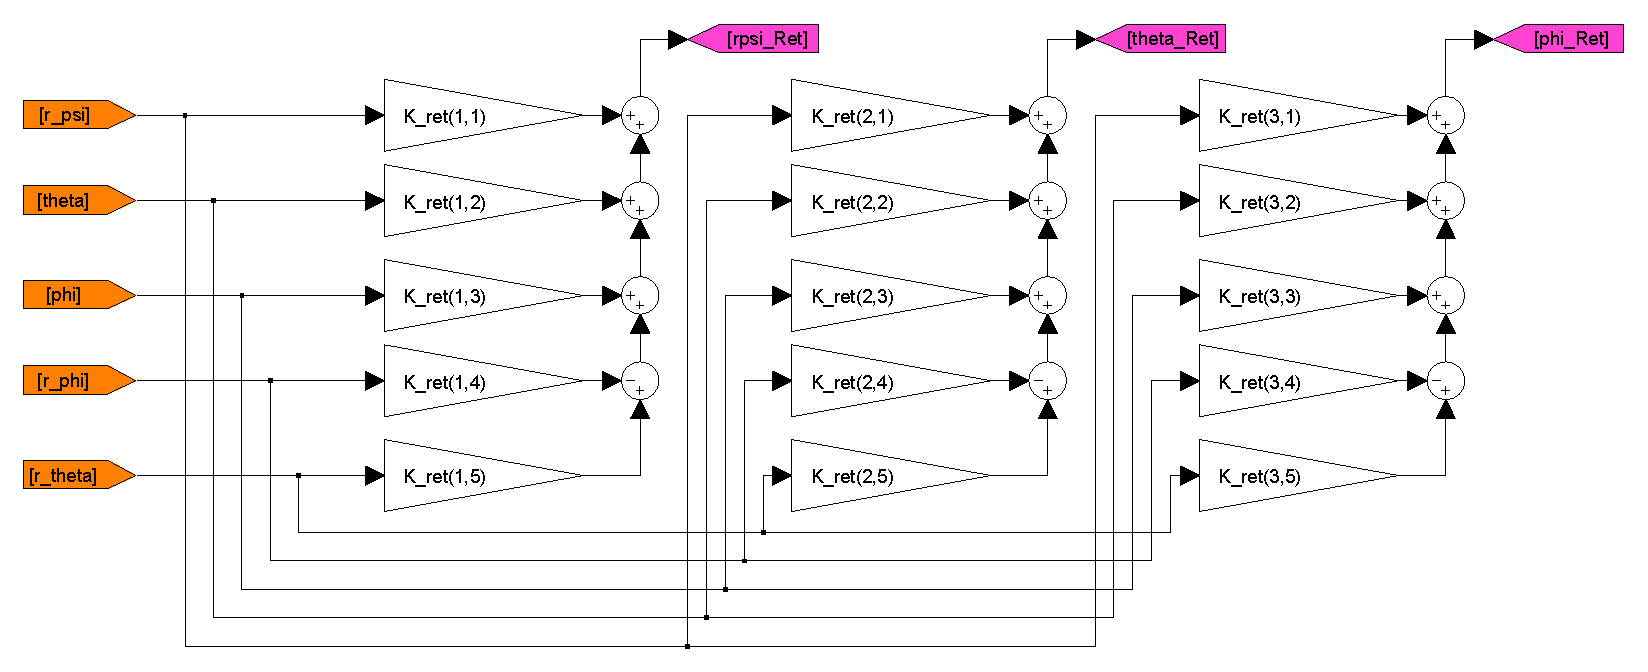
\includegraphics[width=1.00\textwidth]{03_Grafiken/SS_Feedback.pdf}
	\caption{Feedback part of the state space controller}
	\label{fig:SS_Feedback}
\end{figure}

Figure \ref{fig:SS_Feedback} shows the red part of the overview figure \ref{fig:SS_overview}. The input values marked orange, are the measured state variables of the process. The output values marked in magenta, are the added state variables with their specific feedback factors. The calculated matrix (\ref{eq:feedback}) can be written in the gain blocks in this diagram. Now there is maybe some unclarity, because some of those feedback factors are zero and even so there is a gain block for them. The reason is, that if the pole constellation is changed, these calculated values may change from zero to an important value. Another blur is the minus sign in the feedback factors for \textit{rphi}. The answer is very simple - the sensor, measuring this value, is build in the 'wrong way'. So all values have to be flipped.